\documentclass[border=4pt]{standalone}
\usepackage[T1]{fontenc}
\usepackage[scaled]{helvet}\renewcommand{\familydefault}{\sfdefault}
\usepackage{newtxmath}
\usepackage{amsmath}
\usepackage{xcolor}
\usepackage{tikz}
\usetikzlibrary{positioning,arrows.meta,calc,fit,backgrounds}
\definecolor{vblue}{HTML}{2a78d6}
\definecolor{vorange}{HTML}{eb6834}
\definecolor{vink}{HTML}{52514e}
% Generated from report/paper/main.tex (Fig. 2) by the talk build; same diagram for the slides.
\begin{document}
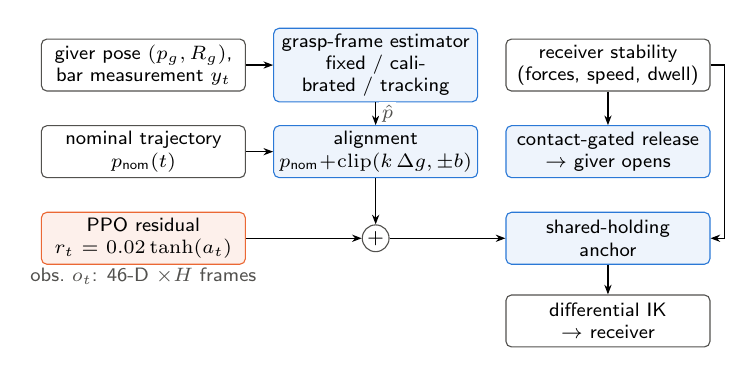
\begin{tikzpicture}[
  font=\scriptsize, >={Stealth[length=3.5pt]},
  blk/.style={draw=vink, rounded corners=2pt, align=center, inner sep=2pt, minimum height=0.66cm,
              text width=2.45cm, fill=white},
  geo/.style={blk, fill=vblue!8, draw=vblue},
  lrn/.style={blk, fill=vorange!10, draw=vorange},
  sum/.style={circle, draw=vink, inner sep=0pt, minimum size=0.34cm, fill=white},
  lab/.style={font=\scriptsize, text=vink, fill=white, inner sep=1pt}]
\node[blk] (sens) at (0,0) {giver pose $(p_g,R_g)$,\\ bar measurement $y_t$};
\node[geo] (est) at (2.95,0) {grasp-frame estimator\\ fixed / calibrated / tracking};
\node[blk] (stab) at (5.9,0) {receiver stability\\ (forces, speed, dwell)};
\node[blk] (nom) at (0,-1.1) {nominal trajectory\\ $p_{\text{nom}}(t)$};
\node[geo] (align) at (2.95,-1.1) {alignment\\ $p_{\text{nom}}+\operatorname{clip}(k\,\Delta g,\pm b)$};
\node[geo] (gate) at (5.9,-1.1) {contact-gated release\\ $\to$ giver opens};
\node[lrn] (ppo) at (0,-2.2) {PPO residual\\ $r_t=0.02\tanh(a_t)$};
\node[sum] (s) at (2.95,-2.2) {$+$};
\node[geo] (anc) at (5.9,-2.2) {shared-holding\\ anchor};
\node[blk] (ik) at (5.9,-3.25) {differential IK\\ $\to$ receiver};
\node[lab, anchor=north] at (ppo.south) {obs.\ $o_t$: 46-D $\times H$ frames};
\draw[->] (sens) -- (est);
\draw[->] (est) -- node[lab, right=1pt]{$\hat p$} (align);
\draw[->] (nom) -- (align);
\draw[->] (align) -- (s);
\draw[->] (ppo) -- (s);
\draw[->] (s) -- (anc);
\draw[->] (anc) -- (ik);
\draw[->] (stab) -- (gate);
\draw[->] (stab.east) -- ++(0.18,0) |- (anc.east);
\end{tikzpicture}
\end{document}
